\textcolor{red}{\textbf{Daqui para baixo: próximos tópicos a desenvolver, rascunho, notas e/ou apontamentos para não esquecer}}

\vspace{1cm}

\vspace{5pt}
\hrule
\vspace{6pt}
%%%%%%%%

%%%%%%%%


Tinkercad as seen in Section \textcolor{red}{Não esquecer de referenciar a secção} could be considered a virtual laboratory and also a online simulator


Virtual laboratories are computer simulations aimed to help students perform a given (simulated) scientific or engineering experiment.

Therefore, within the concept of ``laboratories'' one considers real and remote ones


Therefore, the terms virtual and simulated may be common and may even represent the same system.
With respect to the concept of ``virtual''

\sout{With respect to the concept of ``virtual'' and without losing generality, local simulators and online simulators are considered to fit in this category. (Otherwise the scope of concepts will be duly justified)}

\sout{(which may or may not be a Virtual Laboratory)}.


\begin{itemize}
    \item Multisim online
    \item Falstad
    \item Tinkercad
    \item \textcolor{red}{\textbf{A REVER}}\sout{LabView - Laboratory Virtual Instrumentation Engineering Workbench (?????????)}
    \item vários outros exemplos em     https://www.sciencedirect.com/science/article/pii/S0360131516300227?via%3Dihub - vantagens e desvantagens

\end{itemize}


\begin{itemize}
    \item VISIR
    \item e-Lab
    \item artigo - https://repositorio-aberto.up.pt/bitstream/10216/84571/2/61631.pdf
\end{itemize}

%However, one can also call into discussion another type of resources: online and local simulators.
%: in a normal class multisim is used to first test the circuits
% Enumerar os contexto de aplicação


%https://www.ed.ac.uk/institute-academic-development/learning-teaching/staff/digital-ed/what-is-digital-education

%https://education.ec.europa.eu/focus-topics/digital-education/action-plan?

\vspace{1cm}


(...)
eLearning e stem ou steam
Falar nas Advantages and Disadvantages of Using Various Computer Tools in Electrical Engineering Courses
\vspace{1cm}

Não esquecer o Go-Lab
\vspace{1cm}

%https://www.researchgate.net/publication/343696721_Web_Browser_Electric_Circuit_Simulators_For_Education

Online simulators, such as Multisim, 



%%%%%%%%%%%%%%%%%%%%%%%%%%% TEMP %%%%%%%%%%%%%%%%%%%%%%%%%%%%%%%%%%%%%%%%%
\vspace{1cm}

frase para destacar: Skills not degrees may be the reality of the future.
%https://www.weforum.org/agenda/2019/12/fourth-industrial-revolution-higher-education-challenges/
\vspace{1cm}

Their ability to replicate real components with suficient accuracy and simulate their work in different modes even at the development stage saves time and money for the companies and makes such simulation software extremely popular among the producers of all kind. Creation of breadboards and integrated circuits for pre-implementation testing is too expensive and impractical compared to the virtual simulation
\vspace{1cm}

Simulation has great importance in the field of application of Electronics engineering where electronic engineers or students  can  check  their  models  or  their  models  or  theory  before  applying  for  development practically. In this article, I mainly emphasize some important simulation software tools in the field of electronics and communication engineering. These tools are widely used for numerical simulations and applications. From this article, students will familiarize about these simulation software tools so that they can apply these tools in their own problems and also carry out research work for further development or modifications of these software tools. 

\vspace{1cm}

First, it can provide students an easy access to the complicated energy systems in a virtual environment. Second, the operation principles or performances of the systems can be easily understood and evaluated for undergraduate students without directly solving the difficult mathematical equations. Third, online simulators can be directly used in real research activities for graduate students where the system optimization and evaluation in terms of various design parameters for the system are crucial.

%%%%%%%%%%%%%%%%%%%%%%%%%%% TEMP %%%%%%%%%%%%%%%%%%%%%%%%%%%%%%%%%%%%%%%%%


To be consistent with the concepts explained in the Section \ref{tiposlaboratorios}, simulators, whether remote or local, are considered as part of what are called virtual laboratories.
In fact, the only major difference between a local and remote is how it is accessed: a remote simulator is accessed via web and a local simulator the software is installed in the computer. 


Virtual laboratories present the students with a set of different opportunities, not only as a substitute but also as a complement to the real laboratories. Students can perform dangerous
experiments without endangering themselves. Considering my personal case, in a class with 20 or more students, it is safer to simulate a power circuit using components like TRIACS, DIACS or SCRs. Besides ``The results are always the same. A virtual laboratory allows for independent or collaborative work(\ldots)''\cite{virtuallabng}.

CAsos de estudo e dissertar um pouco sobre os labs

\section {STEM Education}

\vspace{1cm}

\vspace{5pt}
\hrule
\vspace{6pt}

\textcolor{red}{\textbf{PARA FUTURA REFERÊNCIA}}


%%%%%%%%%%%%%%%%%%%%%%%%%% FUTURA REFERÊNCIA %%%%%%%%%%%%%%%%%%%%%%%%%%%%%%%%%%%%

O ensino de engenharia enfrenta diversos desafios, incluindo a necessidade de manter-se atualizado em relação às tecnologias emergentes, bem como preparar os alunos para as demandas do mercado de trabalho em constante evolução. Além disso, a seleção de referências bibliográficas adequadas para o ensino pode ser um desafio, devido à grande quantidade de informações disponíveis e à necessidade de selecionar textos que sejam relevantes e atualizados.

Um dos principais problemas que surgem no ensino de engenharia é a falta de conexão entre a teoria e a prática. Muitas vezes, os alunos são expostos a uma grande quantidade de informações teóricas, mas não têm a oportunidade de aplicar essas informações em projetos práticos. Isso pode levar a uma falta de compreensão sobre como as teorias se aplicam na vida real e pode dificultar a transferência de conhecimento para a prática profissional.

Outro desafio enfrentado pelo ensino de engenharia é a rápida evolução das tecnologias e a necessidade de manter-se atualizado em relação às novas tendências e inovações. A seleção de referências bibliográficas adequadas é essencial para garantir que os alunos estejam expostos às tecnologias e tendências mais recentes. No entanto, a grande quantidade de informações disponíveis pode tornar difícil selecionar as referências mais relevantes e atualizadas.

eLearning has become increasingly important in education in Portugal, especially due to the challenges presented by the COVID-19 pandemic, which forced many educational institutions to adopt distance learning.

One of the main advantages of eLearning is the flexibility it offers. Students can learn at their own pace and schedule, which is particularly useful for those who have other responsibilities, such as work or family care. In addition, eLearning can also be accessed from anywhere, provided there is an internet connection, which allows students to study from home or anywhere else that is convenient for them.

Another advantage of eLearning is that it allows access to a wide variety of learning resources and materials, including videos, texts, interactive activities, discussion forums and more. These resources can be updated and adapted quickly according to the needs of learners and teachers, ensuring that the content is always up-to-date and relevant.

eLearning can also be an effective way to personalise learning, allowing students to focus on areas where they need the most help and move on quickly in areas where they already have knowledge. Students can take online assessments that help determine their skills and knowledge, allowing the teacher to tailor the content and learning activities according to their needs.

For educational institutions in Portugal, eLearning can help reduce costs by eliminating the need for additional physical space and equipment. It can also help reach a wider audience of learners, especially those who do not have access to face-to-face teaching due to geographical, financial or other constraints. eLearning also allows educational institutions in Portugal to provide quality education at a lower cost, allowing more people to access education.

Finally, eLearning can help improve the quality of education in Portugal by enabling students to learn more effectively and efficiently. Teachers can monitor students' progress in real time, providing immediate feedback and adapting content according to students' needs. In addition, eLearning can help foster collaboration between students and teachers, allowing them to work together on projects and group activities regardless of physical location.

In summary, eLearning is an important tool in education in Portugal, allowing educational institutions to provide flexible, personalised and accessible education to a wider audience of learners. Although there are challenges involved in adopting eLearning, the benefits outweigh the challenges, and it is likely that eLearning will continue to be an important part of teaching in Portugal in the future.


\paragraph{PSPICE}
Outro simulador de referência é o \acrfull{pspice}. Este simulador é uma versão \textit{desktop} - \textbf{REVER ESTE TERMO} do \acrshort{spice} que simula o comportamento de circuitos electrónicos e tenta emular tanto os geradores de sinais como o equipamento de medição - multímetros, osciloscópios e analisadores de espetro de frequência. Suporta simulações tanto de circuitos puramente analógicos quanto de circuitos mistos (analógicos e digitais). Além disso, o \acrshort{pspice} possui uma vasta biblioteca de modelos de componentes padrão (analógicas e digitais). Estas características fazem dele uma ferramenta útil para uma vasta gama de aplicações analógicas e digitais\cite{PSpiceSystemSimulation, AboutPSp93:online}. 

\begin{figure}[hbtp]
    \centering
    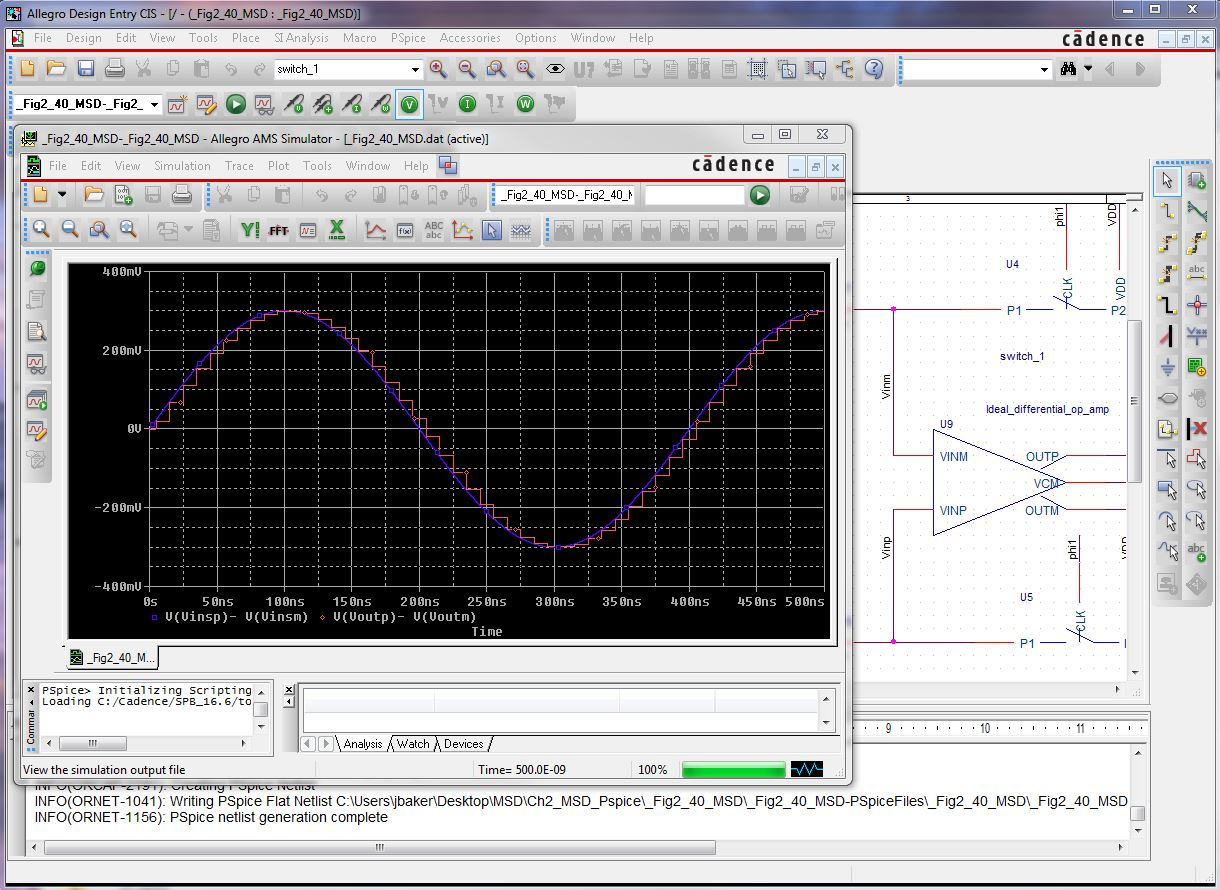
\includegraphics[width=0.9\textwidth]{figures/pspice.jpg}
    \caption{\acrshort{pspice}}
    \label{fig:pspice}
\end{figure}

Com o desenvolvimento quase constante e rápido da tecnologia eletrónica e do \textit{hardware} e \textit{software} informático, a tecnologia de concepção eletrónica substituiu (quase) completamente o método de concepção tradicional baseado na avaliação quantitativa e no circuito de \textit{hardware}. Podemos igualmente referir rapidez com que os computadores podem efetuar cálculos complicados utilizando o modelo de circuito virtual e produzir o resultado da simulação em conformidade com o circuito realista\cite{PSpiceSystemSimulation}.

Em suma, ``os estudantes podem melhorar o desempenho dos projectos tirando partido de uma simulação poderosa para identificar erros mais cedo no fluxo do projeto e reduzir as dispendiosas iterações de protótipos (\ldots)'' \cite{AvoidingCircuitErrorsMultisim}, citando \cite{ApplicationMultisimVirtualLaboratory}. Adicionalmente ``A simulação tem grande importância no domínio da aplicação da engenharia eletrónica, em que os engenheiros electrónicos ou os estudantes podem verificar os seus modelos ou a sua teoria antes de submeterem o projecto para desenvolvimento\cite{ImportantSimSoftware}''.

\paragraph{Caso especial}

\textbf{O FALSTAD NÃO É UM CASO ESPECIAL}

Nas secções anteriores foram abordados os tipos de laboratórios mais comuns e apresentados e discutidos alguns exemplos. No entanto, há um tipo de simulador que vale a pena mencionar e que também é muito utilizado, sendo uma ferramenta que utilizo muito com os meus alunos: \textbf{falstad}\cite{falstad}


%O \textit{Multisim}\cite{multisim} é só um dos laboratórios virtuais aplicado numa base regular em contexto de sala de aula. Outros exemplos passam pelos que já foram mencionados anteriormente: 

% MAS…o VISIR e outros serão laboratórios remotos MESMO QUE a interface seja muito parecida…ou mesmo igual. Há partes do Tinkercad muito parecidas com o visir (a breadboard e componentes virtuais).

% A diferença mais importante é que o laboratório remoto usa componentes REAIS…e a lista de diferenças está na tabela que você próprio colocou. Se reparar, todas as características de um laboratório virtual da tabela são validas para um simulador…mesmo o Falstad.

% Convem que se organize…e no seu estado da arte deverá falar dos 4 tipos…

% Lab Real

% Simulador Local

% Simulador Remoto (que pode ou não ser um Laboratorio Virtual)

% Laboratorio Remoto

% Neste sentido, REMOTO refere-se a operação à distancia. VIRTUAL refere-se a representar “virtualmente” uma coisa real.

% Neste sentido, é até possivel um SIMULADOR LOCAL E VIRTUAL. Uma versão do Tinkercad (ou similar) que corra no seu PC, por exemplo…julgo que existe (ou existiu em tempos)…e seria também um Laboratorio Virtual (e não Remoto).

% Também existem LABORATORIOS REMOTOS que são “virtualmente” diferentes dos seus equivalentes locais…em vez de breadboards e componentes, temos PCBs pre montadas…e na realidade são muito diferentes e menos parametrizáveis do que é possível fazer numa sala de aula…mas são LABS REMOTOS de qq forma…não poderão é ser chamados de virtuais, no contexto acima.

% É a clarificação possível.

% E já agora um aviso…há zonas “cinzentas” em que certas soluções são mistos de simuladores e labs reais e há simuladores que tenham emular o componente real, incluindo erros. No futuro pode ser difícil distinguir…

% Para o seu estado da arte, sugeria que começasse a escrever de acordo com as suas próprias imagens e terminologia. E veja os exemplos que tem…tente pelo menos um de cada. Falstad, Multisim e Tinkercad podem coexistir…convem é que os “classifique” corretamente…
% \par\noindent\rule{\textwidth}{0.4pt}


% Laboratórios Físicos Tradicionais

% Os laboratórios físicos tradicionais são os mais comuns e amplamente utilizados em instituições educacionais e centros de pesquisa. Esses laboratórios são espaços físicos equipados com instrumentos, equipamentos e materiais necessários para realizar experimentos e pesquisas. Eles são fundamentais para disciplinas como química, biologia, física, engenharia e muitas outras.

% A principal vantagem dos laboratórios físicos é a possibilidade de manipulação direta dos materiais e equipamentos, o que proporciona uma experiência prática e tátil que é difícil de replicar em outros tipos de laboratórios. No entanto, a manutenção desses laboratórios pode ser cara, exigindo investimentos significativos em infraestrutura, equipamentos, segurança e materiais consumíveis. Além disso, a disponibilidade de laboratórios físicos pode ser limitada devido a restrições de espaço e recursos financeiros.
%

\paragraph{Enquadramento em contexto de sala de aula}
Na secção \ref{remotelaboratório} - \textbf{REVER REFERÊNCIA}, o impacto dos laboratórios remotos foi abordado de uma forma geral. 

Esta secção abordará o impacto mais específico do \acrshort{visir} na educação.

De acordo com \cite{RemoteLabsImpactVISIR}, e citando \cite{TheVISIRproject} entre outros, sistemas como o \acrshort{visir} partilham algumas vantagens - tal como mencionado na secção \ref{remotelaboratory}. Principalmente:
\begin{itemize}
    \item \textbf{Acessibilidade}: Os laboratórios remotos permitem aos estudantes aceder a equipamento e experiências que estão fisicamente distantes e/ou são demasiado raros ou dispendiosos para estarem disponíveis em laboratórios educativos normais;
    (Aproveitando estas vantagens e colocando-as em contexto da sala de aula - ao longo do capítulo 3 - \textbf{VERIFICAR A REFERÊNCIA AO CAPÍTULO} discutimos algumas das dificuldades associadas à criação e manutenção de um verdadeiro laboratório - é fácil perceber que o \acrshort{visir} tem potencialidades e permite (ou pode permitir...) a realização de experiências que de outra forma não seriam possíveis na sala de aula. Tomando como exemplo uma turma de vinte alunos organizados em pares, seriam necessários 10 osciloscópios, mais 10 geradores de sinais e muitos mais multímetros. A acessibilidade dos laboratórios remotos, e do \acrshort{visir} em particular, ajuda a ultrapassar estes problemas em certas áreas curriculares).
    \item \textbf{Disponibilidade}: As experiências podem estar disponíveis durante períodos alargados e a qualquer hora do dia. As restrições de tempo para a experimentação, repetição ou análise são também mais flexíveis;
    (A disponibilidade também pode ser um problema. Passo a apresentar um exemplo bastante comum nas escolas por onde leccionei: se houver duas turmas dedicadas à eletrónica, é muito difícil que ambas estejam totalmente equipadas com os recursos materiais necessários para o desenvolvimento de experiências. Os laboratórios remotos estão disponíveis 24 horas por dia, 7 dias por semana e permitem uma gestão mais flexível).

    \item \textbf{Segurança}: Os laboratórios remotos são intrinsecamente mais seguros, tanto para o utilizador como para o equipamento, uma vez que estão separados fisicamente e são também mediados pela tecnologia, sendo mais fácil evitar acidentes ou danos no equipamento.
    (Pela minha experiência, este é talvez o fator mais importante que leva à utilização de laboratórios remotos. Embora o \acrshort{visir} não esteja preparado para realizar experiências com eletrónica de potência - mas poderá estar num futuro próximo - são utilizados recursos alternativos como forma de manter a segurança dos alunos e do equipamento).
\end{itemize}

% Sendo assim, foram propostos dois projectos: um centrado no desenvolvimento e controlo do \textit{hardware} e o outro - que diz respeito a esta dissertação - centrado no desenvolvimento do \textit{software}. Pretendia-se utilizar um micro-controlador que, juntamente com um \acrfull{ide} desenvolvido em \acrfull{labview}, pudesse controlar um conjunto de relés. Foram feitos alguns testes com um \gls{arduino} Mega mas dada a complexidade do projecto e, também, uma grande vontade de desenvolver os conhecimentos ao nível do \textit{Python}\footnote{Falaremos um pouco mais sobre esta linguagem nos capítulos seguintes.}, decididu-se avançar com este tipo de linguagem.

% \begin{figure}[hbtp]
%     \centering
%     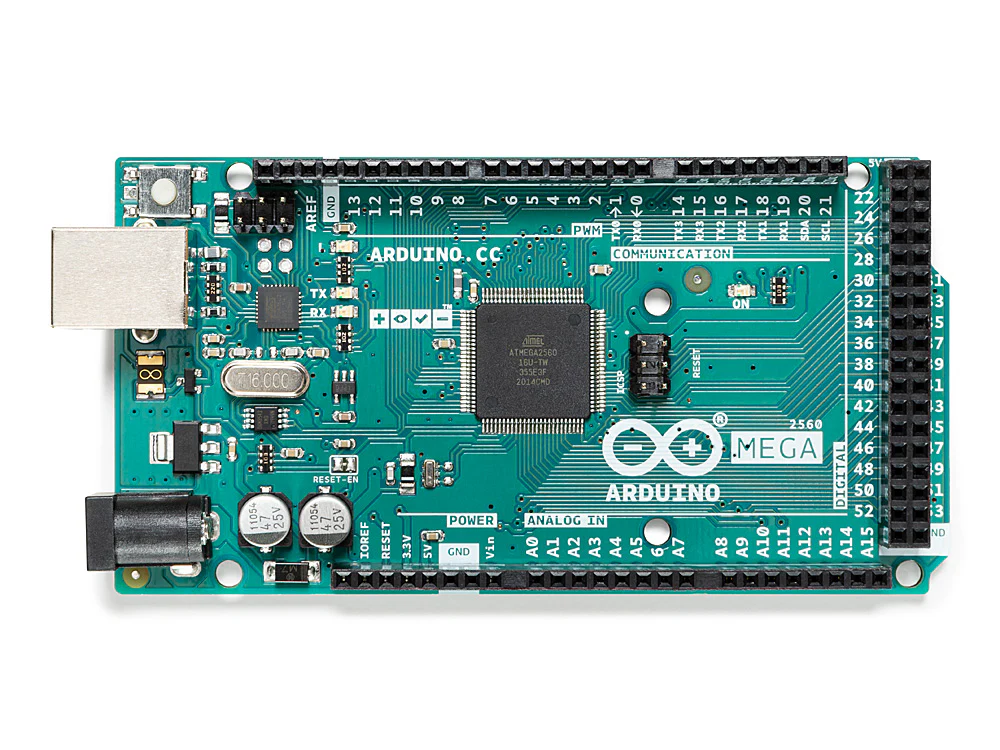
\includegraphics[width=0.6\textwidth]{figures/arduinomega.png}
%     \caption{\textit{Arduino} Mega \cite{ArduinoMega}}
%     \label{fig:arduinomega}
% \end{figure}

% É possível combinar o \textit{Arduino} com o \textit{Python}, mas isso implicaria uma mudança no \textit{firmware}. No entanto, existindo no mercado o \gls{ESP32}, muito mais poderoso decidiu-se, então, avaliar a integração do \gls{ESP32} com o \textit{Python}. Para sermos rigorosos, o uso do \textit{Python} no \gls{ESP32} faz-se através de \textit{MicroPython}, uma implementação leve da linguagem \textit{Python} especificamente projetada para micro-controladores \cite{micropythonesp32}\cite{MicroPythonlib}.
% Após uma análise do \textit{datasheet} \cite{esp32datasheet}, chegou-se à conclusão de que o \gls{ESP32} com \textit{MicroPython} tem limitações de memória. De facto, a memória \textit{flash} varia entre os 4-16 \acrlong{mb}, mais particularmente no modelo ''ESP32-DEVKITC-32E``, que estava disponível para este projecto, que era de 4 \acrshort{mb} \cite{diferencaspython}. 

% \begin{figure}[hbtp]
%     \centering
%     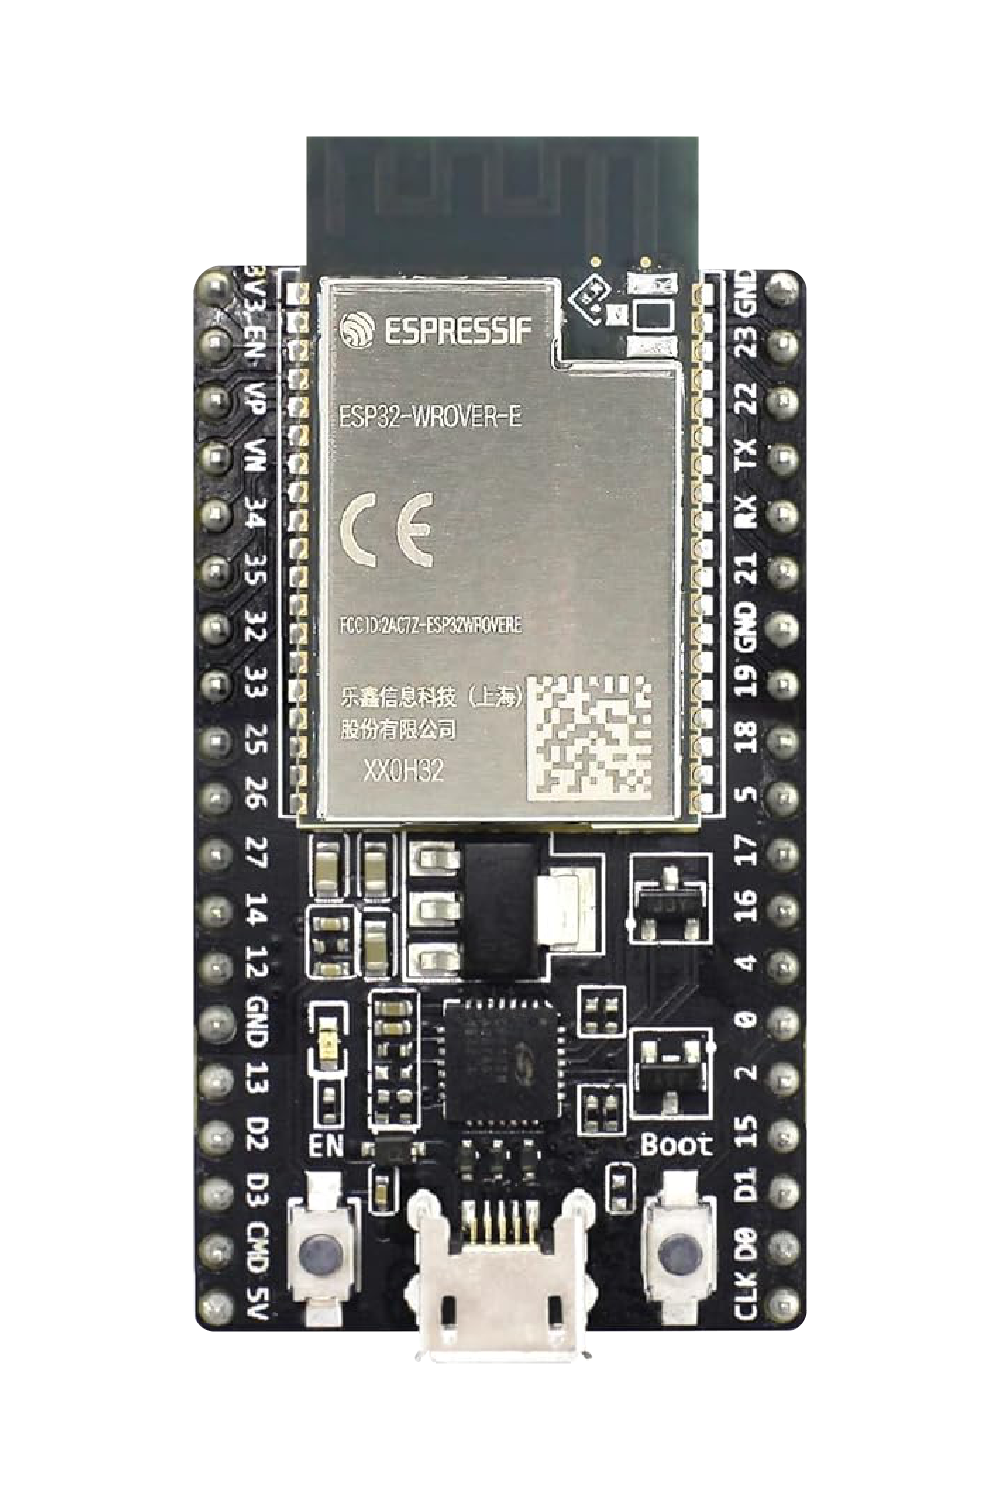
\includegraphics[width=0.4\textwidth]{figures/ESP32-DevKitC_L_0.png}
%     \caption{\textit{ESP32} \cite{ESPDevKit}}
%     \label{fig:ESP32}
% \end{figure}

% Se o objectivo era trabalhar e programar com \textit{Python}, era preciso outro tipo de \textit{hardware}. A escolha seguinte recaiu no \gls{RaspberryPI}\footnote{Nos capítulos seguintes falaremos um pouco mais sobre o \gls{RaspberryPI}}

% \begin{figure}[hbtp]
%     \centering
%     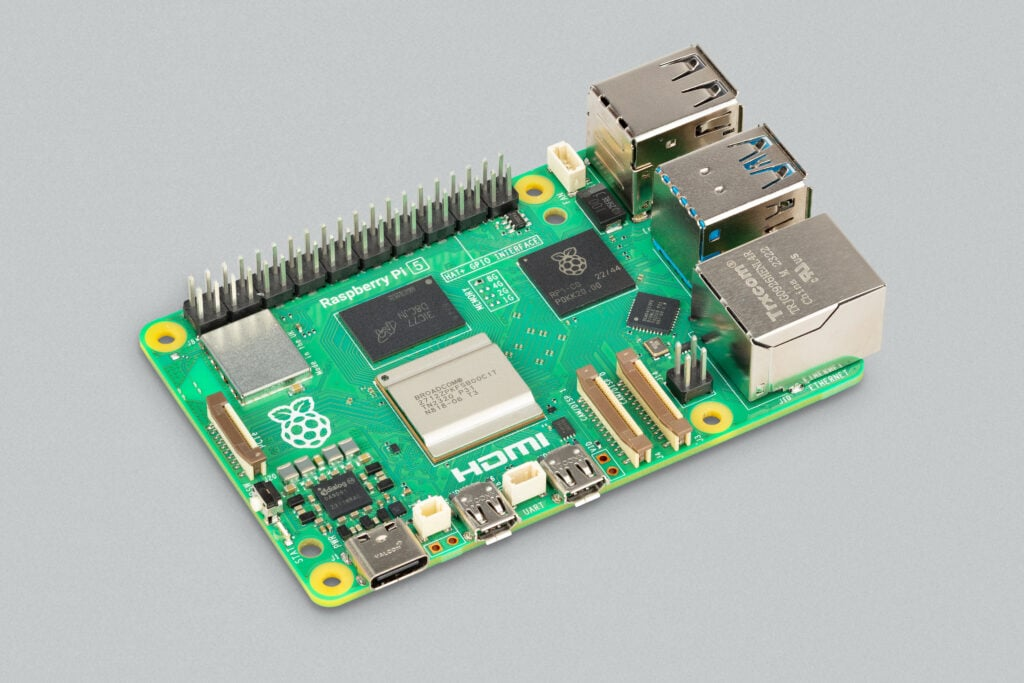
\includegraphics[width=0.6\textwidth]{figures/raspberrypi5.jpg}
%     \caption{\textit{RaspberryPI5} \cite{Raspberrypi5}}
%     \label{fig:Raspberrypi5}
% \end{figure}

% Dentro deste objectivo principal - criar um laboratório remoto como alternativa ao \acrshort{visir}, surgiu um segundo objectivo que se prende com a eliminação do \acrshort{labview}, o \acrshort{ide} inicialmente proposto. De facto, sendo este um \textit{software} proprietário, os preços das diversas versões variam, aproximadamente, entre os 523€ e os 4300€ anuais \cite{labviewpricing}.
% Considerou-se, portanto, que seria uma mais-valia construir um laboratório remoto, cuja linguagem principal (programação e \acrshort{ide}) assentaria em \textit{Python}, controlado por um \gls{RaspberryPI}.

% Estava dado o passo final para o que se viria a tornar o \acrfull{lare}.

% Os objectivos principais foram definidos na Secção \ref{sec: Enquadramento}. Com base neles, podemos formular a pergunta fundamental: 

% \textbf{Será o \acrshort{lare} uma alternativa válida ao \acrshort{visir}?}


Na implementação do \textit{pyVirtualBench} é preciso ter em atenção alguns pormenores que podem levantar potenciais problemas de interpretação e implementação, especialmente na forma com foi desenvolvido a programação referente à Lei de \textit{Ohm}. Como já se viu na Secção \ref{sec:hardware} o \acrshort{virtualbench} é constituído por 5 instrumentos, 4 dos quais utilizados no \acrshort{lare}: Fonte de tensão, gerador de sinal, osciloscópio e multímetro digital.

Outra hipótese seria o uso de variáveis globais. 

Este facto levantou alguns problemas e dificuldades no desenvolvimento do código referente à experiência da Lei de \textit{Ohm}, referidos e explicados mais à frente na Secção XPTO.


\textbf{Eventualmente este parágrafo pode ficar mais à frente quando se abordar a interpretação do diagrama}

Quer isto dizer que, o utilizador ou aluno, parte do valor já conhecido da resistência e constrói o gráfico da Tensão \textit{vs} Corrente, efectuando cinco medições diferentes de cada grandeza. Isto implica que o \textit{script} tenha de ser chamado dez vezes, uma vez que os parâmetros passados para o servidor - \textit{views.py} são diferentes. Outro problema que se levanta é a necessidade de armazenar os valores das variáveis correspondentes às medições. Isto advém do facto de que, entre chamadas do \textit{script}, as variáveis são perdidas.

Sendo assim, na implementação desta experiência, além dos ficheiros \textit{views.py}, \textit{configRelays.py}. \textit{ohm.html}, já referenciados na Secção \ref{sec:organizacao_ficheiros}, foi criado o \textit{configVB.py} que contém as configurações e medições a realizar no \acrshort{virtualbench}, assim como a construção do gráfico final.

JÁ REPETI ESTA MERDA, REVER ESTA PARTE DOS FICHEIROS




Importa referir que o botão ``OK'', além de habilitar os selectores, também ativa e configura previamente a fonte de tensão de \SI{25}{\volt}, conforme descrito na Secção \ref{sec:fontesalimentacao}. Esta abordagem foi adotada para garantir que, no momento das medições, os relés e circuitos integrados já se encontrem devidamente alimentados. Além disso, do ponto de vista do \textit{software} e da estrutura de programação, bem como para a deteção e análise de possíveis erros, considerou-se vantajoso que o envio destes parâmetros e a configuração do \acrshort{virtualbench} fossem realizados logo nesta fase inicial.
O botão ``STOP/RESET'' é responsável por interromper a experiência, desabilitar os selectores e desligar a fonte de alimentação.

%serve também para e ``STOP/RESET'' são implementados com recurso a \textit{JavaScript}, tal como se pode ver na Listagem \ref{lst:okstopreset}.



Para melhor descrever esta experiência e o seu funcionamento no que diz respeito ao \textit{software}, pode dividir-se a explicação em duas etapas: 
\begin{enumerate}
	\item Configuração inicial do \acrshort{virtualbench};
	\item Medição de tensão, corrente e apresentação do gráfico - \textbf{eventualmente três partes com o PI metido ao barulho}. 
\end{enumerate}

Como se pode ver nas Figura \ref{fig:ohm_ctrl}, representadas na Secção \ref{sec:paginas}, a página \textit{ohm.html} é composta por um formulário que permite ao utilizador escolher os parâmetros $V_{CC}$ e R, assim como a medição a efectuar - corrente, tensão e a construção do gráfico.

%\sout{O botão ``OK'' é responsável por habilitar os selectores de parâmetros, assim como habilitar a fonte de 25 do virtualbench. Enquanto que o botão ``STOP/RESET'' é responsável por interromper a experiência e desligar a fonte de alimentação.}

Partindo da sequência anterior, a primeria etapa (1.) - configuração do \acrshort{virtualbench} - é a habilitação dos selectores e a configuração da fonte de \SI{25}{\volt}. Pela análise da Figura \ref{fig:fluxohm}, os parâmetros são enviados da página \textit{ohm.html} para o \textit{script views.py}, da forma como indica a Listagem \ref{lst:exemploenvioparametros}.
%, é feita da forma apresentada na Listagem \ref{lst:exemploenvioparametros}:

\begin{center}
	\begin{minipage}{0.9\linewidth}
		\begin{lstlisting}[language=Html,escapechar=|, caption=Envio de parâmetros da página \textit{ohm.html} para o \textit{script views.py}, label=lst:exemploenvioparametros]
		const booleanParameter = true; |\label{line:trueparameter}|
		const url = `/config_VirtualBench?habilitar_parameter=${booleanParameter.toString()}`
	\end{lstlisting}
	\end{minipage}
\end{center}

\textbf{ESTA MERDA PODE FICAR NOUTRO SÍTIO}

Do lado do servidor - \textit{script views.py} - os parâmetros são recebidos da forma como se pode ver na Listagem \ref{lst:exemplorecepcaoparametros}:
\begin{center}
	\begin{minipage}{1\linewidth}
		\begin{lstlisting}[language=Python,escapechar=|, caption=Recepção dos parâmetros no \textit{script views.py} enviados da página \textit{ohm.html}, label=lst:exemplorecepcaoparametros]
			configOK = request.args.get('habilitar_parameter', 0, bool)|\label{line:configOK}|
		\end{lstlisting}
	\end{minipage}
\end{center}

%Na função \textit{config\_VirtualBench()}, caso os parâmetros não existam, ou se não forem recebidos, linhas \ref{line:vccref} a \ref{line:stopref}, será retornado o valor ``0''.

A Figura \ref{fig:passagemparametros} mostra um exemplo dos valores que o ficheiro \textit{views.py} recebe, quando se carregar no botão ``OK'':
\begin{figure}[hbtp]
	\centering
	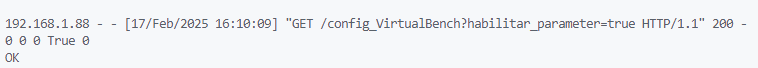
\includegraphics[width=1\textwidth]{figures/exemplo_dados_Ohm.png}
	\caption{Exemplo: passagem de parâmetros}
	\label{fig:passagemparametros}
\end{figure}

O único parâmetro que é passado, é respeitante ao botão ``OK'', que foi definido como \textit{``True''}, representado na Linha \ref{line:trueparameter}, da Listagem \ref{lst:exemploenvioparametros}.

Através da Listagem \ref{lst:recepcaoparametros} pode ver-se que, quando é recebido o parâmetro ``OK'', é chamada a função \textit{OK()}, Linha \ref{line:configOK}, do \textit{script} \textit{configVB.py}. O procedimento é em tudo idêntico quando é seleccionado o parâmetro ``STOP''.

\begin{minipage}{0.9\linewidth}
	\begin{lstlisting}[language=python, escapechar=|, caption=Teste do parâmetro ``OK'' (\ldots e ``STOP'') no ficheiro \textit{views.py}, label=lst:recepcaoparametros]
	(...)
	configOK = request.args.get('habilitar_parameter', None, bool)
	(...)
	if configOK == True:
        configVB.OK() |\label{line:configOK}|  
    elif configSTOP == True:
        configVB.STOP()	
	(...)
	\end{lstlisting}
\end{minipage}


A Figura \ref{fig:experiencialeiohm} representa o esquema completo do processo de execução da experiência. 

\begin{comment}
O procedimento respeitante à configuração inicial do \textit{virtualbench} é realizado quando o utilizador carrega no botão ``OK'', sendo que a comunicação se faz entre três ficheiros: \textit{ohm.html - views.py - configVB.py}. 


	%const booleanParameter = true;
    %const url = `/config_VirtualBench?habilitar_parameter=${booleanParameter.toString()}`;


do Para a primeira etapa, o foco será a configuração comunicação entre a página \textit{ohm.html} e o ficheiro \textit{configVB.py}, representado na Figura \ref{fig:comohmconfigvb}.
\end{comment}

\begin{figure}[hbtp]
	\centering
	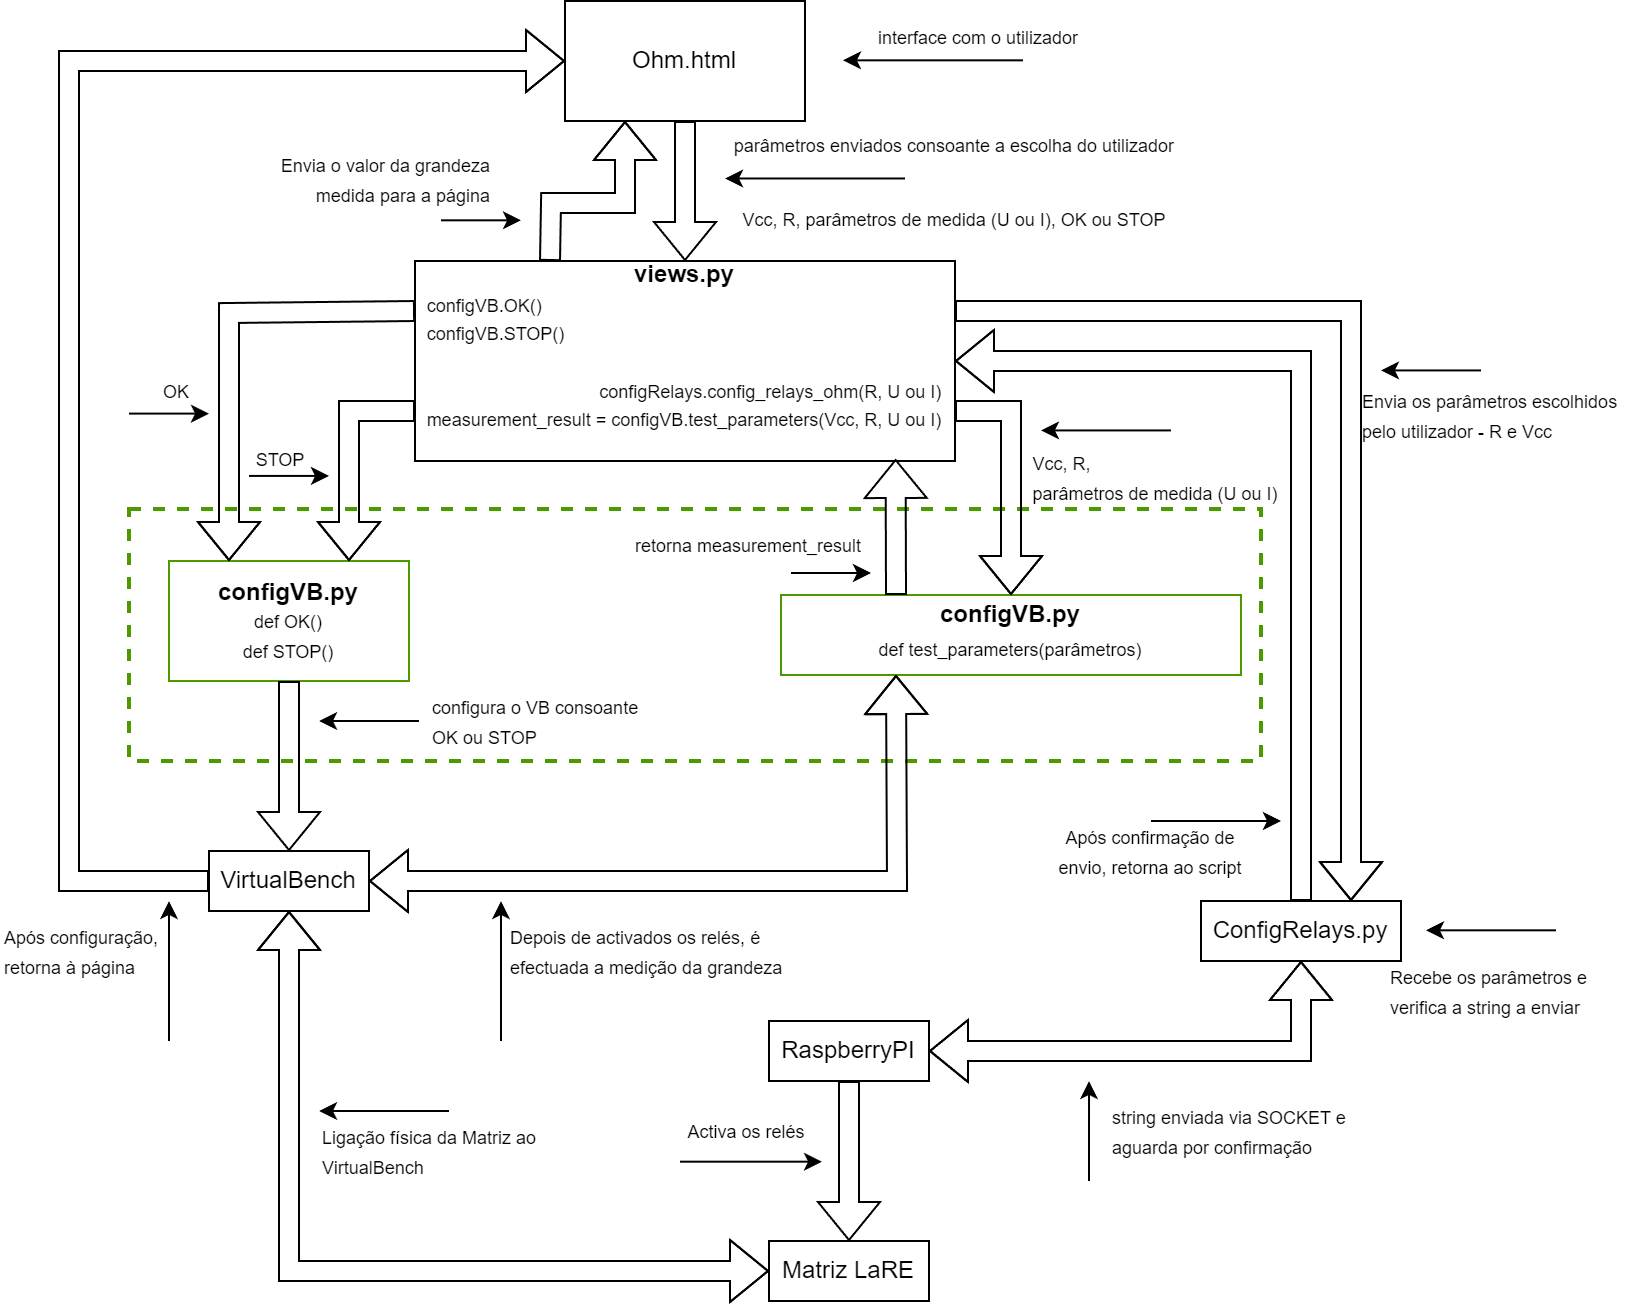
\includegraphics[width=0.8\textwidth]{figures/ohm_diagrama.drawio.png}
	\caption{Diagrama de funcionamento (?) da experiência - Lei de \textit{Ohm}}
	\label{fig:experiencialeiohm}
\end{figure}

\begin{comment}
\begin{figure}[hbtp]
	\centering
	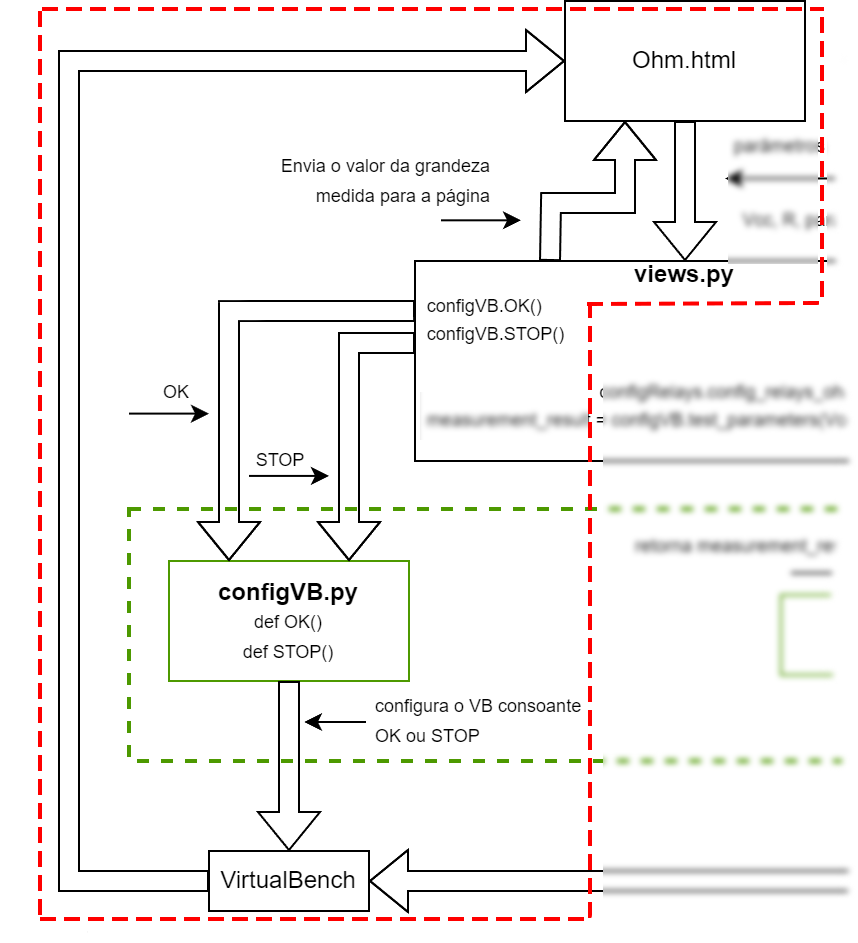
\includegraphics[width=0.6\textwidth]{figures/experiencia_ohm_diagrama.drawio.png}
	\caption{Comunicação \textit{ohm.html} e \textit{configVB.py}}
	\label{fig:comohmconfigvb}
\end{figure}
\end{comment}

%FIQUEI AQUI - COMEÇAR POR DIZER QUE NESTA PARTE ENVOLVE 3 FICHEIROS, TALVEZ DE UMA FORMA MUITO RESUMIDA E DEPOIS PARTIR PARA UMA PARTE RIGOROSA

%EXPLICAR PORQUE SE COLOCOU UM BOTÃO DE OK E STOP/RESET, O PROMENOR DAS FONTES DE12v SEREM PRIMEIRO ACTIVADA AINDA NÃO ESTÁ EXPLICADA EM QQ LADO E FOI POR ISSO QUE SE OPTOU POR COLOCAR OS BOTÕES, AO FAZER RESET, OS ci E OS RELE´S DEIXAM DE ESTAR SOB TENSÃO.
%PORTNATO, O PASSO É, PRIMEIRO ACTIVAR IC E RELES, EFECTUAR MEDIÇÕES. NO FIM DA EXPERIENCIA AO CLICAR EM STOP A FONTE É DESLIGADA

%Entre estes dois ficheiros há envio/recepção de parâmetros.

No entanto, os parâmetros escolhidos só serão efectivamente enviados para o servidor \textit{Flask} - (\textit{views.py}) e a medição efectuada quando:
\begin{enumerate}
	\item Seleccionar o botão ``OK'' que habilita os selectores;
	\item Escolher ambos os parâmetros - $V_{CC}$ e R;
	\begin{enumerate}
		\item Clicar no link ``Medir tensão'' ou ``Medir corrente''.
	\end{enumerate}
\end{enumerate}

%Sequência: 
%1º passo:
%OK - habilita selectores na página HTML e envia o parâmetro para configurar a fonte de 25V, através do ficheiro configVB
%2º passo:
%Seleccionar os parâmetros $V_{CC}$ e R
%3º passo:
%Efectuar medição de tensão ou corrente, através do ficheiro configVB

\paragraph{Configuração inicial do VB} ~\\

O ficheiro \textit{configVB.py} é responsável pela configuração do \acrshort{virtualbench} - E NÃO SÓ - e pela construção do gráfico final. Além das supra-mencionadas inclui ainda as seguintes funções:
\begin{itemize}
	\item \textit{OK()};
	\item \textit{STOP()};
	\item \textit{test\_parameters(Vcc:int, R:int, measure\_parameter:str)};
	\item \textit{plot\_graphic(current\_measurements, voltage\_measurements)}.
\end{itemize}

Como já referido anteriormente, a função ``OK()'' é responsável por activar a fonte de alimentação de \SI{25}{\volt} do \acrshort{virtualbench}, configurá-la para \SI{12}{\volt} e habilitar os selectores dos parâmetros $V_{CC}$ e R. 

% referencia fontesalimentacao Coa fonte de 12V que vai alimentar os integrados e, através do LM317, a fonte de 5V. 

A função ``STOP()'' desactiva e liberta todas as saídas do \acrshort{virtualbench}, assim como os instrumentos e o próprio \acrshort{virtualbench}. Os selectores dos parâmetros $V_{CC}$ e R também são desabilitados.

Na Listagem \ref{lst:exemploOKPS} e Listagem \ref{lst:exemploSTOPPS} pode ver-se um exemplo de configuração da fonte de alimentação e do \textit{RESET}, respectivamente. 

\begin{minipage}{0.9\linewidth}
	\begin{lstlisting}[language=python, escapechar=|, caption=Exemplo de configuração: fonte de alimentação - OK, label=lst:exemploOKPS]
		(...)
		channel = "ps/+25V"
		voltage_level = 12.0
		current_limit = 0.5 
		ps.enable_all_outputs(True)
		ps.configure_voltage_output(channel, voltage_level, current_limit)
		(...)
	\end{lstlisting}
\end{minipage}

\begin{minipage}{0.9\linewidth}
	\begin{lstlisting}[language=python, escapechar=|, caption=Exemplo de configuração: fonte de alimentação - STOP, label=lst:exemploSTOPPS]
		(...)
		if all([ps, dmm, virtualbench]):
		   	ps.enable_all_outputs(False)
        	ps.release()
        	dmm.release()
        	virtualbench.release()
		(...)
	\end{lstlisting}
\end{minipage}

Analisado procedimento de configuração inicial do \acrshort{virtualbench}, o próximo passo (2.) é a medição de tensão e corrente e envio/recepção dos respectivos parâmetros.

\paragraph{Medição da tensão e corrente} ~\\
Na Listagem \ref{lst:exemploenvioparametros} é possível observar como o parâmetro é enviado para o ficheiro \textit{views.py}. No entanto, nesta etapa, são transmitidos três parâmetros: $V_{CC}$, R e o tipo de medição a realizar — corrente ou tensão. O método de envio desses parâmetros é idêntico ao utilizado para um único parâmetro, conforme ilustrado na Listagem \ref{lst:envioparmedidas}.

\begin{minipage}{0.9\linewidth}
	\begin{lstlisting}[language=html, escapechar=|, caption=Envio de parâmetros da página \textit{ohm.html} para \textit{views.py}, label=lst:envioparmedidas]
		(...)
		const parameter = this.dataset.parameter;
		(...)
		const url = `/config_VirtualBench?parameter=${parameter}&Vcc=${Vcc}&R=${Resistance}`;
        fetch(url)
		(...)
	\end{lstlisting}
\end{minipage}

Na Listagem \ref{lst:exemplorecepcaoparametros}, Linhas \ref{line:vccref} a \ref{line:measureref} é possível observar como os parâmetros são recebidos no ficheiro \textit{views.py}.

Após o teste aos parâmetros recebidos, o procedimento pode ser descrito da seguinte forma:
\begin{itemize}
	\item Configurar os relés;
	\item Configurar o \acrshort{virtualbench} e efectuar a medição;
	\item Desligar todos os relés.
\end{itemize}

\textbf{ATENÇÃO - Não esquecer de explicar a rebienga do store e get, nestas funções e o porquê}

\vspace{1cm}

O procedimento pode ser visto na Listagem \ref{lst:procedimentomedicao}, sendo que a Linha \ref{line:configrelays} é responsável por activar os relés, a Linha \ref{line:measureresult} configura o \acrshort{virtualbench}e efectua a medição da grandeza e a Linha \ref{line:stoprelays} desactiva os relés.

\begin{minipage}{0.9\linewidth}
	\begin{lstlisting}[language=python, escapechar=|, caption=Procedimento de medição, label=lst:procedimentomedicao]
		(...)
		configRelays.config_relays_ohm(Resistance, measure_parameter) |\label{line:configrelays}|
		time.sleep(2)
		measurement_result = configVB.test_parameters(Vcc, Resistance, measure_parameter) |\label{line:measureresult}|
		configRelays.config_relays_ohm(0, measure_parameter) |\label{line:stoprelays}|
		(...)
	\end{lstlisting}
\end{minipage}


A configuração dos relés é realizada no ficheiro 

ANALISOU-SE ANTERIORMENTE O PROCEDIMENTO DE OK E STOP-RESET. VAMOS AGORA PARA O ENVIO DOS RESTANTES PARAMENTROS E MEDIÇÕES

!!!!!!!!!! FIQUEI AQUI !!!!!!!!!!
REFERIR, TALVEZ A FONTE DO FLASK, RESPEITANTE AO REQUEST.ARGS

O envio dos restantes parâmetros, $V_{CC}$, R, medição de corrente (I) ou tensão (U) é feito de forma idêntica.

Quando se trata de enviar o resultado das medições para a página \textit{ohm.html}, a comunicação é feita da forma como se pode ver nas Listagens \ref{lst:envioresultados} e \ref{lst:recepcaoresultados}:
\begin{center}
	\begin{minipage}{0.7\linewidth}
		\begin{lstlisting}[language=python, caption=Envio de resultados do servidor (\textit{views.py}) para a página \textit{ohm.html}, label=lst:envioresultados]
			(...)
			return jsonify({'measurement_result': measurement_result})
			(...)
	\end{lstlisting}
	\end{minipage}
\end{center}

\begin{center}
	\begin{minipage}{0.7\linewidth}
		\begin{lstlisting}[language=html, caption=Recepção de resultados na página \textit{ohm.html}, label=lst:recepcaoresultados]
			(...)
			fetch(url)
			.then((response) => response.json())
		.then((data) => {
		  document.getElementById("current-measure").innerHTML =
			data.measurement_result + " mA";
			(...)
			\end{lstlisting}
	\end{minipage}
\end{center}

\subsubsection{O \textit{script configVB.py}}
\textbf{Este script poderá eventualmente ficar enquadrado numa secção a criar, denominada ``Descrição dos scripts'' ou então, na descrição da experiência lei de ohm.}

\hrule
\hrule

Como se pode ver na Figura , os selectores estão desabilitados e os relés nao estão alimentados porque isso é feito através da fonte do VB e do LM317

Já se viu (\textbf{refirerir a secção}) que na experiência da Lei de \textit{Ohm}, o utilizador selecciona os valores da tensão e resistência através de um formulário, representado na página \textit{ohm.html} da forma como se pode ver na Listagem \ref{lst:formularioescolha}.

\begin{center}
	\begin{minipage}{0.7\linewidth}
		\begin{lstlisting}[language=html, caption=Formulário de escolha na página \textit{ohm.html},label=lst:formularioescolha]
			(...)
			<div style="display: inline-block; width: 200px">
      <select id="selectVcc" disabled>
        <option value="0">Seleccionar V<sub>cc</sub>:</option>
        <option value="1">1</option>
        <option value="2">2</option>
        <option value="3">3</option>
        <option value="4">4</option>
        <option value="5">5</option>
      </select>
    </div>

    <div style="display: inline-block; width: 200px">
      <select id="selectR" disabled>
        <option value="0">Seleccionar R:</option>
        <option value="1">1</option>
        <option value="2">1.1</option>
        <option value="3">1.5</option>
      </select>
			(...)
	\end{lstlisting}
	\end{minipage}
\end{center}

O primeiro a ser chamado, como pode ser vist
\begin{figure}[hbtp]
	\centering
	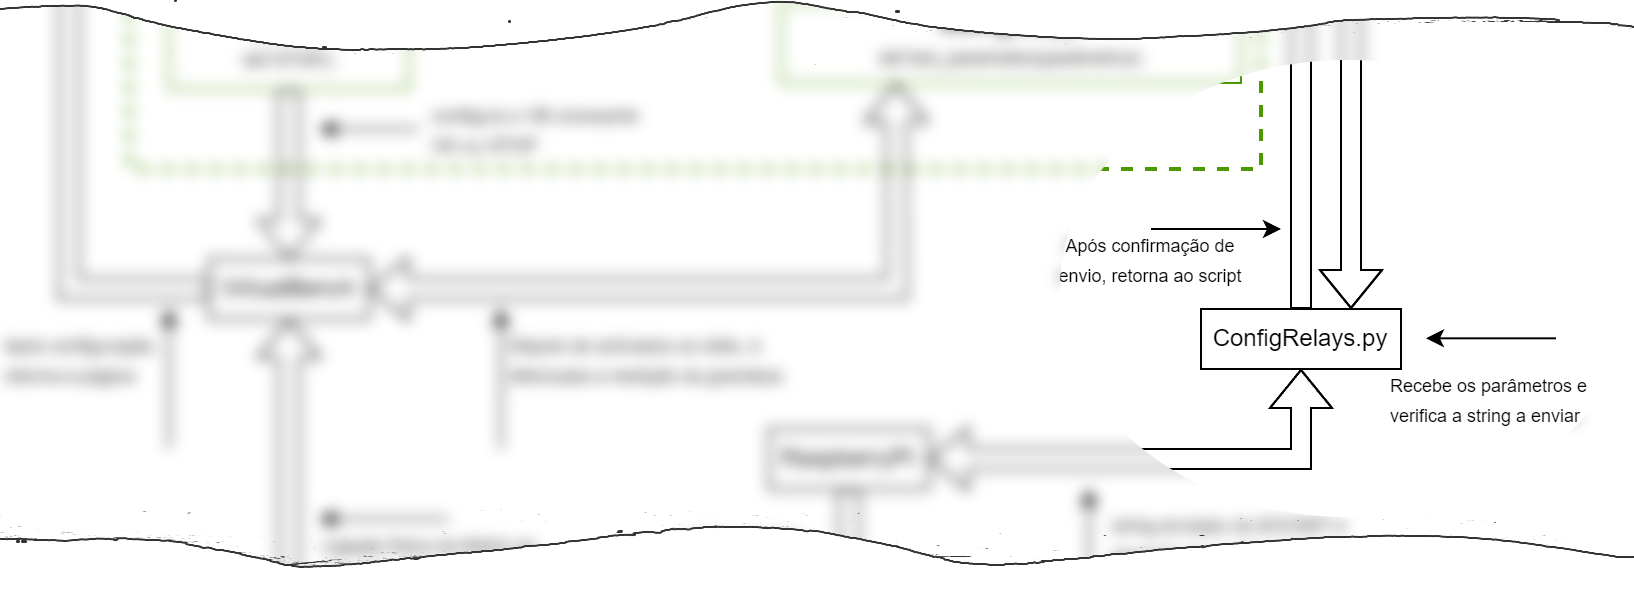
\includegraphics[width=1\textwidth]{figures/ohm_diagramaCUTRelay.drawio.png}
	\caption{\textit{Script configRelays.py}}
	\label{fig:cutconfigRelays}
\end{figure}

\section{qualquer coisa que ainda não sei o quê}

Após análise e estudo da informação presente no \textit{site} do \textit{Flask} e nos tutoriais mencionados em cima, definiu-se e implementou-se a página de autenticação no ficheiro \textit{auth.py}, tal como pode ser visto na Figura \ref{fig:paglogin}:

\begin{figure}[hbtp]
	\centering
	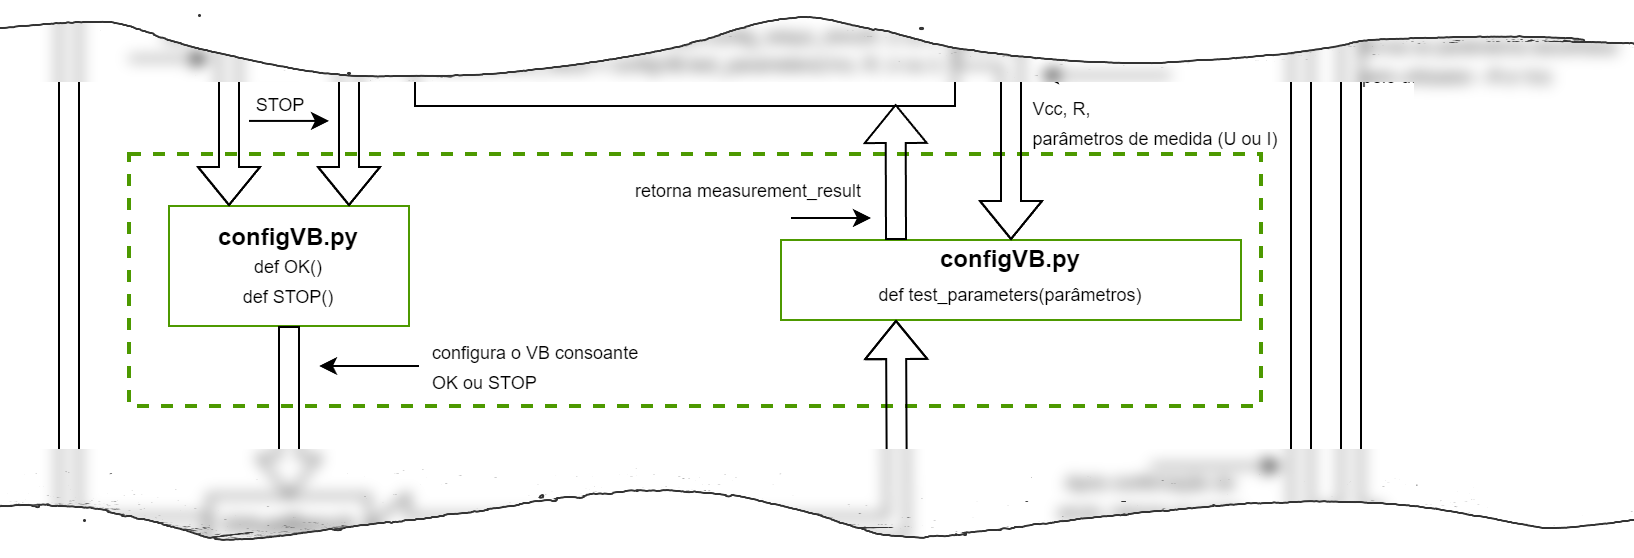
\includegraphics[width=1\textwidth]{figures/ohm_diagramaCUT.drawio.png}
	\caption{caralho}
	\label{fig:diagramaCUT}
\end{figure}

Além da rota definida para o \textit{login}, as outras rotas definidas no ficheiro \textit{auth.py} foram as \textit{sign-up} e \textit{logout}. A estrutura base da função \textit{login}, representada na Listagem \ref{lst:exemplologin}, é idêntica para as restantes, sendo que ``/\textit{login''} representa a rota especificada, dentro da função há o código especifico inerentes a cada função e o \textit{return render\_template} indica qual a página a ser renderizada.

Pode-se, no entanto, referir as principais funções que permitem a medição de tensão, corrente ou sinal no osciloscópio \cite{pyvirtualbench} - \textbf{NOTA: valerá a pena esta parte? PROF}:

\begin{itemize}
	\item Multímetro digital - \acrshort{dmm}
		\begin{itemize}
			\item \textit{dmm.read()} - efectua a medição de tensão ou corrente, consoante os parâmetros definidos na função de configuração: dmm.configure~\textunderscore measurement(DmmFunction.DC~\textunderscore VOLTS, True, 10) ou dmm.configure~\textunderscore measurement(DmmFunction.DC~\textunderscore CURRENT, True, 10);
		\end{itemize}
	\item Osciloscópio
	\begin{itemize}
		\item \textit{mso.read~\textunderscore analog~\textunderscore digital~\textunderscore u64()} - efectua a medição de sinal, sendo que a configuração é automática: \textit{mso.auto~\textunderscore setup()};
	\end{itemize}
	\item Gerador de sinal
	\begin{itemize}
		\item \textit{fgen.run()} - inicia o gerador de sinal, após as configurações iniciais:\\fgen.configure~\textunderscore waveform(fgen~\textunderscore function, frequency, amplitude, offset);
	\end{itemize}
\end{itemize}

\begin{minipage}{0.9\linewidth}
	\centering
	\begin{lstlisting}[language=Python, escapechar=|, caption=Configuração da fonte de \SI{6}{\volt}, label=lst:limiteI]
		try:
			# Power Supply Configuration
			channel = "ps/+6V" |\label{line:channel}|
			voltage_level = Vcc |\label{line:voltagelevel}|
			current_limit = 0.5 |\label{line:currentlimit}|
		(...)
	\end{lstlisting}
\end{minipage}

\textbf{NOTA: Esta parte seguinte talvez deva ficar na parte de software. Aqui só o que diz respeito ao IDE na óptica do utilizador.}
Pela consulta da Listagem \ref{lst:exemplogerador}, pode ver-se que o gerador de sinal está configurado com uma amplitude de \SI{10}{\volt} e um \textit{duty-cycle} de 50\%. Tal como referido na Secção (...), após a aquisição do instrumento, este é configurado com os valores definidos nas Linhas (...) e iniciado.

\begin{minipage}{0.9\linewidth}
	\begin{lstlisting}[language=Python,escapechar=|, caption=Exemplo configuração do gerador de sinal - \textit{mixed\textunderscore signal\textunderscore oscilloscope.py}, label=lst:exemplogerador]
	waveform_function = Waveform.SINE
	amplitude = 10.0      # 10V
	dc_offset = 0.0       # 0V
	duty_cycle = 50.0     # 50% duty cycle
	(...)
	\end{lstlisting}
\end{minipage}

A Listagem \ref{lst:exemplomso} apresenta a configuração dos osciloscópio que segue o mesmo padrão (?) dos restantes instrumentos. 

O \textit{setup} é configurado de forma automática e as restantes configurações, Linhas a a, foram retiradas do exemplo \textit{mso\_simple\_example.py}. Por fim, é realizada a aquisição do sinal na Linha (...).

\begin{minipage}{0.9\linewidth}
	\begin{lstlisting}[language=Python,escapechar=|, caption=Exemplo configuração do oscilscópio - \textit{mixed\textunderscore signal\textunderscore oscilloscope.py}, label=lst:exemplomso]
	
	(...)
	mso.auto_setup()
	(...)
	# Start the acquisition.  Auto triggering is enabled to catch a misconfigured trigger condition.
	mso.run()
	
	# Read the data by first querying how big the data needs to be, allocating the memory, and finally performing the read.
    analog_data, analog_data_stride, analog_t0, digital_data, digital_timestamps, digital_t0, trigger_timestamp, trigger_reason = mso.read_analog_digital_u64()
	(...)
	\end{lstlisting}
\end{minipage}

A implementação completa das configurações do gerador de sinal e osciloscópio estão definidas no ficheiro ``mixed\textunderscore signal\textunderscore oscilloscope.py''. Como referido na Secção \ref{sec:configmedicaoes}, o código foi retirado dos exemplos aquando da instalação do \textit{pyVirtualBench} e modificado consoante as necessidades do projecto.

De facto, a transformação digital já alterou os postos de trabalho e, a nível mundial, a indústria, os produtos e as modalidades de ensino. Pode concluir-se, então, da importância dos laboratórios na educação ou, neste caso particular, do laboratório de eletrónica, principalmente em contexto de sala de aula.